\documentclass[a4paper,12pt]{article}

\usepackage{alltt, fancyvrb, url}
\usepackage{graphicx}
\usepackage[utf8]{inputenc}
\usepackage{float}
\usepackage{hyperref}
\usepackage[italian]{babel}
\usepackage[table]{xcolor}
\usepackage{array}
\usepackage{multirow}
\usepackage{titlesec}
\usepackage{listings}
\usepackage[italian]{cleveref}
\usepackage{acronym}
\usepackage{subcaption}

\renewcommand{\thesection}{\arabic{section}}

\sloppy
\setlength{\parindent}{0pt}

\title{\textbf{Gestione dei rischi}}
\author{}
\date{}

\begin{document}
\maketitle
\tableofcontents

\newpage

\section{Analisi dei rischi}
Effettuiamo un'analisi dei rischi precedentemente individuati, valutando la probabilità e l'impatto di ciascun rischio,
dopo averli categorizzati. Nella \Cref{tab:risk_analysis} sono riportati i rischi individuati, specificando le
probabilità e gli impatti come Low (L), Medium (M) o High (H).
\begin{table}[!htb]
    \centering
    \begin{tabular}{|p{0.03\textwidth}|p{0.15\textwidth}|p{0.15\textwidth}|p{0.37\textwidth}|p{0.18\textwidth}|p{0.12\textwidth}|}
        \hline
        \textbf{ID} & \textbf{Categoria} & \textbf{Scope Triangle} & \textbf{Rischio} & \textbf{Probabilità} & \textbf{Impatto} \\ \hline
        1 & Tecnico & Qualità & In alcune zone con basso segnale, gli aggiornamenti provenienti dalle colonnine di
        ricarica potrebbero subire dei ritardi & M & M \\ \hline
        2 & Tecnico & Qualità & Introduzione di bug nel software delle colonnine di ricarica & L & H \\ \hline
        3 & Tecnico & Scope & Incertezza nella realizzazione di un algoritmo per generare il percorso ottimizzato & H & H \\ \hline
        4 & Tecnico & Tempo & Ritardi nella schedula a causa dell'integrazione con sistemi esistenti & M & M \\ \hline
        5 & Project management & Tempo & Attese del completamento della milestone 2 per poter iniziare l'applicazione mobile & M & M \\ \hline
    \end{tabular}
    \caption{Analisi dei rischi.}
    \label{tab:risk_analysis}
\end{table}

\newpage

\section{Mitigazione dei rischi}
Per ogni rischio individuato, in base alla valutazione della combinazione tra probabilità e impatto (vedi
\Cref{fig:risk_matrix}), si decide quale strategia adottare. Nella \Cref{tab:risk_mitigation} sono riportate le
strategie di mitigazione dei rischi individuati.

\begin{figure}[!htb]
    \centering
    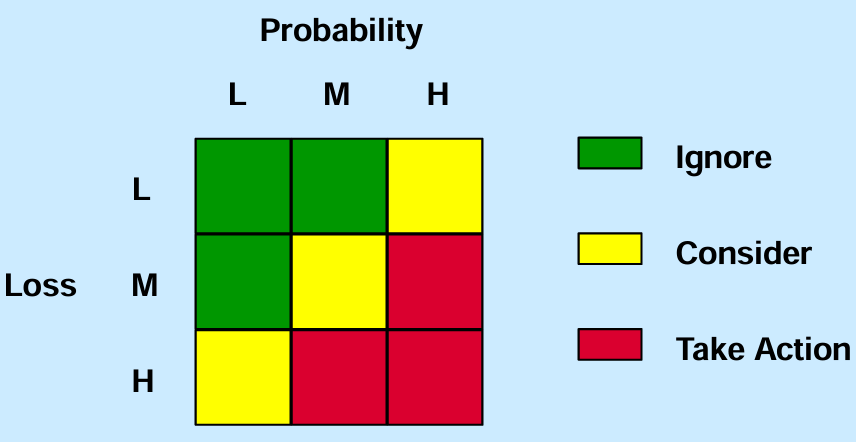
\includegraphics[width=0.7\textwidth]{images/risk_matrix.png}
    \caption{Matrice dei rischi.}
    \label{fig:risk_matrix}
\end{figure}

\begin{table}[!htb]
    \centering
    \begin{tabular}{|p{0.03\textwidth}|p{0.2\textwidth}|p{0.2\textwidth}|p{0.57\textwidth}|}
        \hline
        \textbf{ID} & \textbf{Valutazione} & \textbf{Strategia} & \textbf{Descrizione} \\ \hline
        1 & Consider & Mitigazione & Aggiunta di avvisi per rendere l'utente consapevole del problema. \\ \hline
        2 & Consider & Mitigazione & Utilizzo di test anti-regressione durante lo sviluppo. \\ \hline
        3 & Take action & Mitigazione & Utilzzo di Kanban per aumentare la flessibilità nella gestione della schedula. \\ \hline
        4 & Consider & Accettazione & Si accetta il rischio di eventuali ritardi dovuti all'integrazione. \\ \hline
        5 & Consider & Piano di contingenza & Le risorse in attesa dello stesso ambito possono aiutare quelle in
        ritardo, dato che possiedono la conoscenza necessaria del progetto. Oppure effettuare cambiamenti alla
        schedula. \\ \hline
    \end{tabular}
    \caption{Strategie di mitigazione dei rischi.}
    \label{tab:risk_mitigation}
\end{table}

\end{document}